%  LaTeX support: latex@mdpi.com
%=================================================================
% Suppress "xcolor already loaded" warning from TikZ (MDPI class pre-loads xcolor)
\PassOptionsToPackage{table}{xcolor}
\documentclass[jimaging,article,submit,pdftex,moreauthors]{Definitions/mdpi}

%=================================================================
% MDPI internal commands - do not modify
\firstpage{1}
\makeatletter
\setcounter{page}{\@firstpage}
\makeatother
\pubvolume{1}
\issuenum{1}
\articlenumber{0}
\pubyear{2026}
\copyrightyear{2026}
\datereceived{ }
\daterevised{ }
\dateaccepted{ }
\datepublished{ }

%=================================================================
% Full title of the paper (Capitalized)
\Title{Diagnosing Label Noise Robustness via Pseudo-Label Noise Amplification Cascade (PNAC)}

% Authors, for the paper (add full first names)
\Author{Sagy Gabay \textsuperscript{1} and Chen Giladi \textsuperscript{1,*}}

% MDPI internal command: Authors, for metadata in PDF
\AuthorNames{Sagy Gabay and Chen Giladi}

% Affiliations / Addresses
\address{%
\textsuperscript{1} \quad Department of Mechanical Engineering, Sami Shamoon College of Engineering, Ashdod, Israel}

% Contact information of the corresponding author
\corres{Correspondence: chengi1@sce.ac.il}

% Abstract
\abstract{Label noise is pervasive in real-world image classification datasets, yet assessing its impact without costly relabeling remains challenging. We introduce Pseudo-Label Noise Amplification Cascade (PNAC), a diagnostic framework that monitors how iterative pseudo-labeling affects validation performance. Through controlled experiments on a three-class ultrasound dataset with synthetic noise (\texorpdfstring{$\rho$}{rho} from 0.00 to 0.60, \texorpdfstring{$n = 3$}{n = 3} seeds), we identify two cascade outcomes: \emph{amplification}, where confident pseudo-labels propagate errors, and \emph{starvation}, where no pseudo-labels pass the confidence threshold. A \emph{robustness horizon} emerges: mean F1 remains above 0.92 up to 40\% noise, with sharp transition at 45\%. The iterative cascade achieves up to \texorpdfstring{$40\times$}{40x} lower cross-seed standard deviation than single-pass evaluation and higher effect-size separation (Hedges' \texorpdfstring{$g = 6.00$}{g = 6.00} vs.\ 1.24). A throughput cliff provides early warning of regime transition. We develop a theoretical model of cascade stability and validate it on synthetic data, showing that PNAC distinguishes label noise from inherent task difficulty. A sensitivity study confirms the horizon persists across confidence thresholds. PNAC requires only a small clean validation set for multi-signal data-quality triage; findings are based on \texorpdfstring{$n = 3$}{n = 3} seeds, so effect-size estimates are indicative.}

% Keywords
\keyword{label noise; pseudo-labeling; semi-supervised learning; data quality; ultrasound imaging; robustness diagnosis}

% Enable external BibTeX bibliography
\externalbibliography{yes}

% TikZ for flowcharts
\usepackage{tikz}
\usetikzlibrary{shapes,arrows,positioning,calc,decorations.pathreplacing}

% Algorithm environment
\usepackage[ruled,linesnumbered,vlined]{algorithm2e}

% Table with automatic column width
\usepackage{tabularx}
\usepackage{multirow}

\setlength{\headheight}{20pt}
\addtolength{\topmargin}{-8pt}

\begin{document}

\section{Introduction}
High-quality labels are foundational to supervised learning, yet real-world labels are often imperfect~\cite{frenay2014classification,song2022survey}. In medical imaging, operator fatigue, ambiguous visual cues, and inconsistent annotation protocols introduce label errors~\cite{karimi2020deep,joskowicz2019interobserver,tajbakhsh2020interrater}. Sampling bias in other applied domains and inter-annotator variability in crowdsourced annotation produce similar corruption~\cite{northcutt2021confident}. Such label noise alters learning dynamics and can cause models to memorize incorrect mappings~\cite{arpit2017closer,zhang2021understanding}.

This paper addresses not only how to train under noise but also how to \emph{diagnose} a pipeline's robustness to it. A reliable diagnostic tells practitioners whether to collect more labels, invest in a data audit, or adopt noise-robust training strategies.

\begin{figure}[H]
\centering
\begin{tikzpicture}[
    node distance=1.2cm,
    box/.style={rectangle, draw, rounded corners, minimum width=2cm, minimum height=1cm, align=center, fill=white},
    arrow/.style={->, >=stealth, thick},
    every node/.style={font=\small}
]

% Left: Dataset node
\node[box, fill=gray!10] (dataset) {Labeled Dataset\\$D_L$\\{\scriptsize (Unknown Quality)}};

% Middle: PNAC Diagnostic box
\node[box, right=1.2cm of dataset, fill=blue!10, minimum width=2.3cm] (pnac) {PNAC\\Diagnostic};

% Looping arrow for iteration
\draw[arrow, looseness=4] (pnac.north) to[out=60, in=120] node[above, font=\scriptsize] {Iterate} (pnac.north);

% Output signals
\node[box, right=1.4cm of pnac, fill=green!15, minimum width=2.0cm, minimum height=1.5cm] (signals) {Diagnostic\\Signals\\{\scriptsize F1 trajectory}\\{\scriptsize Pseudo-label $|P_t|$}};

% Decision nodes on far right
\node[box, fill=green!20, minimum width=1.7cm, minimum height=0.7cm]
    at ($(signals.east)+(1.8cm,-0.8)$) (standard) {Standard\\Training};
\node[box, fill=red!20, minimum width=1.7cm, minimum height=0.7cm]
    at ($(signals.east)+(1.8cm,0.8)$) (audit) {Data Audit /\\Robust Training};

% Arrows connecting elements
\draw[arrow] (dataset) -- (pnac);
\draw[arrow] (pnac) -- (signals);
\draw[arrow, green!60!black] (signals.east) -- ++(0.5cm,0) |- (standard.west);
\draw[arrow, red!60!black] (signals.east) -- ++(0.5cm,0) |- (audit.west);

\end{tikzpicture}
\caption{Conceptual overview of PNAC as a robustness diagnostic. A labeled dataset of unknown quality is fed through the PNAC diagnostic, which iteratively applies pseudo-labeling while monitoring validation F1 and pseudo-label throughput. The resulting signals guide practitioners to either proceed with standard training (stable F1, active cascade) or invest in data auditing (degraded F1 or cascade starvation).}
\label{fig:pnac_overview}
\end{figure}

Pseudo-labeling is a standard semi-supervised technique in which a model trained on labeled data assigns labels to unlabeled examples~\cite{lee2013pseudo}. Under ideal conditions, pseudo-labeling improves accuracy by incorporating confidently predicted unlabeled examples into training~\cite{xie2020unsupervised}. Under noisy conditions, however, pseudo-labels amplify mistakes: a model trained on corrupted labels produces confident errors that propagate across iterations, creating a confirmation bias loop~\cite{arazo2020pseudo}. Rather than treating this amplification as a problem to mitigate, PNAC leverages it as a diagnostic signal.

As Figure~\ref{fig:pnac_overview} illustrates, PNAC operationalizes this insight through the following protocol. A baseline model trains on the noisy labeled set, pseudo-labels an unlabeled pool via a confidence threshold and test-time augmentation (TTA), and retrains on the expanded set. Under low noise, performance remains stable. Under high noise, errors either propagate through confident mislabeling (\emph{amplification}) or the cascade halts because no predictions exceed the threshold (\emph{starvation}). Both outcomes reveal information about underlying data quality.

This paper makes six contributions:
\begin{enumerate}
\item We introduce PNAC, a diagnostic framework that assesses label-noise robustness by monitoring validation performance and pseudo-label throughput under iterative pseudo-labeling.
\item We derive an analytical model of cascade stability based on pseudo-label precision dynamics, yielding the self-correcting condition ($q_{t+1} > 1 - \varepsilon_t$) and validating it against direct measurements of latent quantities.
\item We identify two distinct cascade outcomes---\emph{amplification} (confidently wrong) and \emph{starvation} (cascade halts due to uncertainty)---and characterize a \emph{robustness horizon} through controlled experiments on an ultrasound dataset ($n = 3$ seeds per condition).
\item We provide empirical evidence that the iterative cascade achieves up to $40\times$ lower cross-seed standard deviation than single-pass evaluation.
\item We present a confidence threshold study ($\tau \in \{0.70, 0.80, 0.90, 0.95\}$) confirming that the robustness horizon persists across thresholds.
\item We conduct validation on a controlled synthetic dataset confirming that PNAC correctly distinguishes label noise from inherent task difficulty.
\end{enumerate}

\section{Problem Formulation and Design Goals}
\subsection{Problem Formulation}
This work assumes access to a labeled dataset $D_L$ collected through a standard annotation workflow. The labels may be imperfect, but the magnitude and structure of the errors are unknown. The goal is to assess pipeline robustness to label noise without relabeling the entire dataset.

Formally, we view the observed label $\tilde{y}$ as a noisy version of an unobserved true label $y$. The noise process may be random, such as uniform label flips; systematic, involving consistent confusion between specific classes; or instance-dependent. PNAC does not attempt to recover the full noise transition matrix. Instead, it provides diagnostic signals revealing whether pseudo-labeling would fail on the dataset.

The diagnostic must be practical in applied settings. Many applied teams can afford a small clean validation split but not a large relabeling effort, and many pipelines have access to large unlabeled pools---a standard assumption in semi-supervised learning~\cite{sohn2020fixmatch,xie2020unsupervised}. Clinical imaging systems, for example, generate data continuously, but only a fraction receives expert labels. PNAC leverages this unlabeled pool to amplify and expose noise effects.

\subsection{Design Goals}
PNAC is designed around four practical goals. First, the method requires only a small clean validation set beyond the potentially noisy training labels, keeping annotation cost minimal. Second, it reuses standard training code with only minor additions, ensuring compatibility with existing pipelines. Third, rather than producing a single scalar, PNAC outputs trajectories of F1 over iterations and pseudo-label counts, enabling richer multi-signal interpretation. Fourth, the diagnostic distinguishes between qualitatively different cascade outcomes (amplification vs.\ starvation).

\subsection{Choice of Evaluation Metric}
The default metric in PNAC is macro-F1 because it accounts for class imbalance and exposes uneven performance across classes~\cite{sokolova2009systematic,song2022survey}. When one class dominates, accuracy can remain deceptively high even as minority classes are misclassified. Macro-F1 averages per-class F1 scores, so the diagnostic signal reflects degradation across all classes.

Table~\ref{tab:notation} summarizes the notation used throughout.

\begin{table}[H]
\caption{Notation summary.}
\label{tab:notation}
\centering
\small
\begin{tabular}{@{}c p{0.78\linewidth}@{}}
\toprule
Symbol & Definition \\
\midrule
$D_L$ & Labeled training set (may contain label noise) \\
$D_U$ & Unlabeled pool \\
$V$ & Clean validation set \\
$\rho$ & Noise rate: fraction of training labels corrupted \\
$\tau$ & Confidence threshold for pseudo-label selection \\
$T$ & Number of pseudo-labeling rounds \\
$K$ & Number of TTA runs \\
$P_t$ & Pseudo-label set added at iteration $t$ \\
$D_t$ & Cumulative training set at iteration $t$ ($D_L \cup P_1 \cup \cdots \cup P_{t-1}$) \\
$\text{F1}_t$ & Validation macro-F1 at iteration $t$ \\
$\Delta$F1 & $\text{F1}_0 - \text{F1}_T$ (positive $=$ degradation) \\
$\beta$ & Fitted decay rate: $-\hat{b}$, where $\hat{b}$ is the OLS slope of $\text{F1}_t$ on $t$ \\
$\varepsilon_t$ & Effective corruption rate in $D_t$ \\
$q_t$ & Pseudo-label precision at iteration $t$ \\
$r_t$ & Throughput ratio: $|P_{t+1}| / |D_t|$ \\
$\rho^*$ & Robustness horizon (Section~\ref{sec:horizon_criterion}) \\
$\theta_F, \theta_\sigma$ & Horizon criterion thresholds for mean F1 and cross-seed SD \\
\bottomrule
\end{tabular}
\end{table}

\section{Related Work}
\subsection{Learning with Noisy Labels}
Research on noisy-label learning spans robust loss functions, curriculum learning, sample selection, and semi-supervised formulations~\cite{frenay2014classification,song2022survey,zhang2023noisy_longtail}. Robust loss functions reduce the influence of suspected label errors by reweighting or modifying the loss~\cite{zhang2018gce,wang2019sce}. Sample selection methods identify likely clean samples using loss statistics or agreement between models~\cite{han2018coteaching,yu2019coteaching_plus,wei2022selffiltering}. Hybrid approaches~\cite{li2020dividemix} combine sample selection with semi-supervised learning on the suspected noisy samples. These methods improve classification performance in the presence of noise. PNAC is complementary: it is not a training method but a diagnostic that helps decide whether to apply robust training.

\subsection{Pseudo-Labeling and Semi-Supervised Learning}
While the methods above aim to \emph{mitigate} noise during training, pseudo-labeling-based approaches interact with noise differently: they can inadvertently \emph{propagate} it. Pseudo-labeling assigns labels to unlabeled data based on model predictions, often with a confidence threshold~\cite{lee2013pseudo}. Modern variants~\cite{sohn2020fixmatch} combine augmentation with confidence filtering. These pseudo-labeling methods generally assume that high-confidence predictions are likely correct. In contrast, PNAC repurposes the confidence threshold to detect how the pseudo-labeling mechanism responds to potentially corrupted initial labels.

\subsection{Data Auditing}
A complementary line of research \emph{diagnoses} data quality before or alongside model training. Data auditing aims to quantify dataset quality without fully relabeling~\cite{northcutt2021confident,zhu2024unmasking}. Training-dynamics-based approaches~\cite{swayamdipta2020datamaps} characterize individual examples along axes of predictive confidence and label agreement but require specialized per-sample analysis and may incur significant computational overhead. PNAC offers an alternative that uses only the existing labeled set and an unlabeled pool.

In summary, existing noise-robust methods focus on \emph{mitigating} noise during training but do not assess whether mitigation is needed; pseudo-labeling methods assume clean initial labels and treat noise propagation as a side effect rather than a signal; and data auditing tools require per-sample analysis or noise-model estimation. PNAC addresses these gaps by repurposing the pseudo-labeling cascade itself as a diagnostic: the cascade's response to noise---stable, starving, or amplifying---reveals dataset quality without requiring noise-model assumptions, per-sample scoring, or any modification to the training pipeline beyond iterative retraining.

\section{Methods}

\subsection{PNAC Pipeline Overview}
The PNAC diagnostic proceeds in iterations. At each iteration $t$, the method (1)~trains a classifier $f_t$ on the current training set $D_t = D_L \cup P_1 \cup \cdots \cup P_{t-1}$, (2)~evaluates $f_t$ on a clean validation set $V$ to obtain macro-F1, (3)~applies $f_t$ to the unlabeled pool $D_U$ with TTA, (4)~selects high-confidence predictions as pseudo-labels $P_{t+1}$, and (5)~records the validation F1 and pseudo-label count $|P_{t+1}|$. Figure~\ref{fig:pnac_overview} illustrates this workflow.

Algorithm~\ref{alg:pnac} formalizes the complete procedure.

\begin{algorithm}[H]
\caption{PNAC Diagnostic Protocol}
\label{alg:pnac}
\SetAlgoLined
\SetKwInOut{Input}{Input}
\SetKwInOut{Output}{Output}
\SetKwFunction{Train}{TrainClassifier}
\SetKwFunction{Evaluate}{EvaluateMacroF1}
\SetKwFunction{PseudoLabel}{PseudoLabelWithTTA}

\Input{Labeled set $D_L$, Unlabeled pool $D_U$, Clean validation set $V$, Confidence threshold $\tau$, TTA runs $K$, Pseudo-labeling rounds $T$}
\Output{F1 trajectory $\{\text{F1}_t\}_{t=0}^{T}$, Pseudo-label counts $\{|P_t|\}_{t=1}^{T}$}

\BlankLine
$D_0 \leftarrow D_L$\;
$U \leftarrow D_U$\;

\For{$t = 0$ \KwTo $T$}{
    $f_t \leftarrow$ \Train{$D_t$}\;
    $\text{F1}_t \leftarrow$ \Evaluate{$f_t$, $V$}\;

    \If{$t < T$}{
        $P_{t+1}, U \leftarrow$ \PseudoLabel{$f_t$, $U$, $\tau$, $K$}\;
        $D_{t+1} \leftarrow D_t \cup P_{t+1}$\;
        Record $|P_{t+1}|$\;
    }
}

\Return{$\{\text{F1}_t\}_{t=0}^{T}$, $\{|P_t|\}_{t=1}^{T}$}
\end{algorithm}

\subsection{Pseudo-Label Selection with TTA}
To reduce variance in confidence estimates, PNAC applies TTA during pseudo-label selection. For each unlabeled sample $x$, we generate $K$ augmented versions and average the softmax outputs:
\begin{equation}
\bar{p}_t(y \mid x) = \frac{1}{K} \sum_{k=1}^{K} f_t(y \mid a_k(x)),
\end{equation}
where $a_k(x)$ denotes the $k$-th augmentation. A pseudo-label is assigned only if $\max_y \bar{p}_t(y \mid x) \geq \tau$.

\subsection{Diagnostic Signals}
PNAC produces two primary diagnostic signals. The first is the \emph{F1 trajectory}, the sequence $\{\text{F1}_0, \text{F1}_1, \ldots, \text{F1}_T\}$, which reveals how validation performance evolves. We use $\text{F1}_0$ and $\text{F1}_T$ throughout; Appendix tables use the aliases $\text{F1}_{\text{init}}$ and $\text{F1}_{\text{final}}$ for readability. Key derived metrics from the F1 trajectory are:
\begin{itemize}
\item $\Delta$F1 $= \text{F1}_0 - \text{F1}_T$: overall degradation. Positive values indicate degradation; negative values indicate improvement.
\item $\min_t \text{F1}_t$: the worst-case performance during the cascade.
\item Fitted decay rate $\beta = -\hat{b}$, where $\hat{b}$ is the ordinary least-squares slope of $\text{F1}_t$ on iteration index $t \in \{0,\ldots,T\}$. The sign is negated so that $\beta > 0$ indicates degradation (declining F1) and $\beta < 0$ indicates improvement. For example, if F1 drops by 0.02 per iteration on average, $\hat{b} = -0.02$ and $\beta = 0.02$.
\end{itemize}

The second signal is \emph{pseudo-label throughput} $\{|P_1|, |P_2|, \ldots, |P_T|\}$, which reveals cascade dynamics. Growing $|P_t|$ with stable F1 indicates healthy pseudo-labeling. Growing $|P_t|$ with declining F1 is consistent with \emph{amplification}, where confident pseudo-labels can propagate errors. Finally, $|P_t| \approx 0$ for multiple iterations indicates \emph{starvation}, where the model is too uncertain to produce pseudo-labels above $\tau$. An intermediate outcome, \emph{mild cascade}, occurs when pseudo-labels are produced in moderate numbers without F1 collapse, indicating marginal rather than runaway error propagation.

\subsection{Robustness Horizon Criterion}
\label{sec:horizon_criterion}
We define the \emph{robustness horizon} $\rho^*$ as the smallest noise rate $\rho$ at which two conditions are simultaneously satisfied:
\begin{enumerate}
\item \textbf{Performance condition:} mean cascade $\text{F1}_T$ (across seeds) falls below a threshold $\theta_F$.
\item \textbf{Instability condition:} cross-seed $\text{SD}(\text{F1}_T)$ exceeds a threshold $\theta_\sigma$.
\end{enumerate}
The joint requirement prevents false triggers: a small mean drop with low variance reflects graceful degradation, not a phase transition. The two-condition structure of the criterion is general; the specific threshold values are dataset-dependent. For illustration, we set $\theta_F = 0.92$ and $\theta_\sigma = 0.03$ \emph{post hoc} from the observed stable-regime statistics: $\theta_F$ equals the lowest mean cascade F1 in the stable regime ($\rho \leq 0.40$; Table~\ref{tab:main_results}), and $\theta_\sigma$ is the smallest round value exceeding the highest stable-regime cross-seed SD (0.025 at $\rho = 0.20$). Because these illustrative thresholds are derived from the same experiment they evaluate, they cannot independently validate the horizon location; we therefore report a sensitivity sweep over $\theta_F \in \{0.87, 0.90, 0.92\}$ and $\theta_\sigma \in \{0.02, 0.03, 0.05\}$ in Section~\ref{sec:robustness_horizon} as the primary evidence that the horizon is robust to threshold choice. Applying this criterion to a new dataset requires setting $\theta_F$ and $\theta_\sigma$ from an independent calibration set or from domain-specific performance standards.

\subsection{Theoretical Analysis: Cascade Stability}
\label{sec:theory}
We develop an analytical model (our derivation) to characterize when the pseudo-labeling cascade is self-correcting versus self-reinforcing, building on the noisy-label and pseudo-labeling frameworks of~\cite{frenay2014classification,song2022survey,arazo2020pseudo}. Let $\varepsilon_t$ denote the \emph{effective corruption rate}---the fraction of incorrect labels in $D_t$ at iteration $t$. Initially, $\varepsilon_0 = \rho$, the injected noise rate. At each iteration, the model trained on $D_t$ generates pseudo-labels $P_{t+1}$ with precision $q_{t+1}$---the fraction of pseudo-labels exceeding $\tau$ that match the true labels~\cite{rizve2021defense}. This model rests on three assumptions:
\begin{enumerate}[label=(\roman*)]
\item The confidence threshold $\tau$ is fixed across iterations.
\item $q_{t+1}$ is measured only over pseudo-labels that exceed $\tau$.
\item Corruption propagation is modeled as a weighted average over the cumulative training set, in which all samples contribute equally regardless of when they were added.
\end{enumerate}
Under these assumptions, the effective corruption evolves as:
\begin{equation}
\label{eq:corruption_dynamics}
\varepsilon_{t+1} = \frac{\varepsilon_t \cdot |D_t| + (1 - q_{t+1}) \cdot |P_{t+1}|}{|D_t| + |P_{t+1}|}.
\end{equation}

Equation~\eqref{eq:corruption_dynamics} is a weighted average: the new corruption rate combines existing corrupted samples, diluted or concentrated by newly added pseudo-labels. Define the \emph{throughput ratio} $r_t = |P_{t+1}| / |D_t|$, the relative size of the newly added pseudo-label batch. Substituting into Equation~\eqref{eq:corruption_dynamics} yields:
\begin{equation}
\label{eq:corruption_throughput}
\varepsilon_{t+1} = \frac{\varepsilon_t + (1 - q_{t+1}) \cdot r_t}{1 + r_t}.
\end{equation}

From Equation~\eqref{eq:corruption_throughput}, the cascade is \textbf{self-correcting} when $\varepsilon_{t+1} < \varepsilon_t$, which requires:
\begin{equation}
\label{eq:self_correcting}
q_{t+1} > 1 - \varepsilon_t.
\end{equation}

That is, pseudo-label precision must exceed the fraction of \emph{correct} labels in the current training set (i.e., $q_{t+1} > 1 - \varepsilon_t$). When the self-correcting condition holds, pseudo-labels are ``cleaner'' than the existing data, and the cascade dilutes corruption. When it fails, corruption accumulates. Note that Equations~\eqref{eq:corruption_throughput}--\eqref{eq:self_correcting} assume $r_t > 0$. In the \emph{starvation} case ($r_t = 0$, no pseudo-labels exceed $\tau$), Equation~\eqref{eq:corruption_throughput} reduces to $\varepsilon_{t+1} = \varepsilon_t$: corruption is frozen at its current level. The self-correcting condition is then vacuous because no new labels enter the training set.

At a critical noise rate $\rho^*$, the initial model's pseudo-label precision $q_1$ falls below $1 - \rho^*$, and the cascade becomes self-reinforcing. Our experiments place $\rho^*$ between $0.40$ and $0.45$ for the ultrasound dataset (Table~\ref{tab:main_results}). This analysis provides a theoretical basis for the empirically observed \emph{robustness horizon}: below $\rho^*$, the cascade is stable; above it, corruption either accumulates---amplification, when $r_t > 0$---or the model produces no pseudo-labels---starvation---when $r_t = 0$.

Whether starvation or amplification occurs depends on whether the corrupted model retains high confidence or becomes uncertain. The resulting confidence level varies with random initialization and batch ordering, explaining the seed-dependent bifurcation observed empirically.

We hypothesize that the split between cascade outcomes is mediated by confidence calibration~\cite{guo2017calibration}. A miscalibrated model that remains overconfident under noise passes incorrect pseudo-labels through the threshold (amplification). Conversely, a model whose softmax outputs reflect its degraded accuracy fails to exceed $\tau$ (starvation). This mechanism is consistent with the observed bifurcation pattern but remains a conjecture; measuring expected calibration error (ECE) across seeds to test this hypothesis is a priority for future work (Section~\ref{sec:conclusion}).

The synthetic experiments (Section~\ref{sec:mechanism_validation}) \emph{experimentally validate} the self-correcting condition under controlled conditions: at $\rho = 0.30$, measured pseudo-label precision $q_1 \approx 0.95 > 1 - 0.30 = 0.70$, and corruption decreases from 0.30 to 0.21 (self-correcting). At $\rho = 0.50$, $q_1 \approx 0.19 < 1 - 0.50 = 0.50$, and corruption persists at $\varepsilon_t \approx 0.52$ (self-reinforcing). The corruption dynamics model also explains the throughput cliff (\emph{hypothesis-generating} for real data, where $q_t$ is not directly observable): as noise increases, model confidence decreases, reducing $r_t$ toward zero. At sufficiently high noise, $r_t = 0$ (starvation) and $\varepsilon_{t+1} = \varepsilon_t$---corruption is frozen but not amplified.

\section{Experimental Setup}

\subsection{Dataset}
\label{sec:dataset}
We evaluated PNAC on a three-class ultrasound dataset for femoral vessel localization. The \textbf{Background} class indicates no vessel is present, \textbf{Center} denotes a vessel centered in the image, and \textbf{Not Center} denotes a vessel that is present but off-center. The classes are exactly balanced: each class contains 2,204 labeled images (6,612 total). Using a fixed manifest with seed 42 and approximate split ratios of 70/15/15, we partitioned each class proportionally into a labeled training set $D_L$ of 4,626 samples (1,542 per class), a clean validation set $V$ of 990 samples (330 per class), and a held-out test set of 996 samples (332 per class). The test set was not used during PNAC diagnostics; post-hoc evaluation on the test set (Appendix~\ref{sec:test_generalization}) confirms that validation-based diagnostics generalize. A separate unlabeled pool $D_U$ of 35,654 samples comprises the remaining unannotated acquisitions.

Table~\ref{tab:data_splits} summarizes the dataset splits with absolute counts and provenance.

\begin{table}[H]
\caption{Data dictionary for dataset splits.}
\label{tab:data_splits}
\centering
\small
\begin{tabular}{@{}l r r l l@{}}
\toprule
Split & Total & Per Class & Labels & Provenance \\
\midrule
$D_L$ (train) & 4,626 & 1,542 & Expert (+ synthetic noise) & 70\% of labeled pool \\
$V$ (validation) & 990 & 330 & Expert (clean) & 15\% of labeled pool \\
Test & 996 & 332 & Expert (clean) & 15\% of labeled pool \\
$D_U$ (unlabeled) & 35,654 & --- & None & Unannotated acquisitions \\
\bottomrule
\end{tabular}
\end{table}

Figure~\ref{fig:dataset_samples} shows representative images from each class. The visual similarity between Center and Not Center---both contain a bright needle shaft against similar tissue---motivates the use of PNAC to assess whether annotation noise between these classes affects downstream models.

\begin{figure}[H]
\centering
\includegraphics[width=0.9\linewidth]{figures/dataset_samples.pdf}
\caption{Representative ultrasound images from each class. \textbf{Background}: no vessel or needle visible. \textbf{Center}: needle centered in the image. \textbf{Not Center}: needle present but off-center. The visual similarity between Center and Not Center makes this pair most susceptible to annotation noise.}
\label{fig:dataset_samples}
\end{figure}

A single board-certified expert sonographer with over five years of clinical ultrasound experience annotated all labeled samples ($D_L$, $V$, test). A second reviewer verified the annotations, and disagreements were resolved by consensus, following standard practice~\cite{joskowicz2019interobserver}. Splits were assigned at the image level. Each image corresponds to a separate, independent phantom acquisition session, so image-level splitting does not introduce session leakage.

We applied noise injection \emph{only} to $D_L$ and retained the original expert labels for $V$ throughout all experiments, ensuring that diagnostic signals are measured against a clean reference.

\subsection{Noise Injection Protocol}
To evaluate PNAC under controlled conditions, we injected synthetic uniform noise into $D_L$ at rates $\rho \in \{0.00, 0.10, 0.20, 0.30, 0.40, 0.45, 0.50, 0.55, 0.60\}$. For each noise rate, we randomly flipped a fraction $\rho$ of training labels to one of the remaining incorrect classes with equal probability (symmetric noise). The condition $\rho = 0.00$ served as the clean baseline. For each seed, we generated the corrupted label set once before the cascade began and held it fixed across all $T$ iterations (fixed-noise protocol). Different seeds produced different corruption realizations of $D_L$, but within a single run no labels were re-sampled, ensuring that observed degradation reflects cascade dynamics rather than re-sampling drift.

\subsection{Implementation Details}
\label{sec:implementation}
We used a ResNet-18 architecture~\cite{he2016resnet} with ImageNet~\cite{deng2009imagenet} pretraining, trained for five epochs per iteration with the Adam optimizer~\cite{kingma2015adam} at a learning rate of $10^{-3}$. Five epochs per iteration was chosen because the pretrained feature extractor required only minor adaptation on this small target dataset ($|D_L| = 4{,}626$); in preliminary experiments, validation F1 stabilized by epoch 3--4 across noise rates. Formal epoch-level loss curves were not logged, so we cannot rule out marginal under-training; however, any such effect would be uniform across noise conditions and would not alter the comparative diagnostic patterns that PNAC relies on.

The cascade used $T = 5$ pseudo-labeling rounds (with baseline evaluation at $t=0$), a confidence threshold $\tau = 0.85$, and $K = 3$ TTA runs. Five iterations were chosen because the key diagnostic patterns---throughput cliff, F1 degradation, and seed-dependent bifurcation---stabilized by $t = 3$--$4$ in preliminary experiments; additional iterations did not change the qualitative conclusions. All configurations were evaluated across three random seeds (42, 123, 456). With $n = 3$ seeds per condition, inferential uncertainty is substantial. We therefore report population standard deviation (SD, dividing by $n$) throughout, because the three seeds constitute the complete set of evaluated conditions rather than a sample drawn from a larger population. With $n = 3$, sample SD (dividing by $n-1$) would be ${\approx}18\%$ larger, but neither estimate is statistically precise at this sample size; we treat effect-size estimates as indicative rather than precise.

Measured F1 and SD values are reported to three decimal places; Hedges' $g$ to two; noise rates $\rho$ and thresholds ($\tau$, $\theta_F$, $\theta_\sigma$) to two; and throughput counts as integers. Synthetic-data F1 values (Section~\ref{sec:mechanism_validation}) are reported to two decimal places, reflecting the lower inherent precision of that experiment.

All experiments ran on a single NVIDIA RTX 3090 GPU. We fixed seeds for all random number generators (Python, NumPy, PyTorch) but enabled cuDNN benchmark mode for performance. This mode can introduce minor non-determinism across hardware configurations~\cite{pytorch2024reproducibility}. To quantify this residual variance, we verified that re-running the same seed on the same hardware produced F1 values within $\pm$0.002 of the original run; cross-hardware reproducibility was not tested.

\section{Results}

\subsection{Robustness Horizon}
\label{sec:robustness_horizon}
A clear \emph{robustness horizon} emerged from the experimental results (Table~\ref{tab:main_results}): pseudo-labeling maintained stable performance (mean F1 $>$ 0.92, $n = 3$ seeds) up to $\rho = 0.40$, with a sharp transition to instability at $\rho = 0.45$.

Under the illustrative post-hoc thresholds (Section~\ref{sec:horizon_criterion}, $\theta_F = 0.92$, $\theta_\sigma = 0.03$), the first noise rate satisfying both conditions is $\rho^* = 0.45$ (mean F1 = 0.841, SD = 0.058), consistent with the theoretical estimate of $\rho^* \approx 0.40$--$0.45$ (Section~\ref{sec:theory}). Because these thresholds were derived from the same data (see Section~\ref{sec:horizon_criterion}), this point estimate alone cannot confirm the horizon location. The sensitivity sweep below serves as the primary evidence.

To assess robustness to threshold choice, we varied both thresholds: for $\theta_F \in \{0.87, 0.90, 0.92\}$ and $\theta_\sigma \in \{0.02, 0.03, 0.05\}$, the criterion consistently yields $\rho^* = 0.45$. The horizon shifts to $\rho^* = 0.20$ only under the most restrictive pair ($\theta_F \geq 0.93$ and $\theta_\sigma \leq 0.02$), which flags the modest SD = 0.025 at $\rho = 0.20$ as instability. The stability of $\rho^* = 0.45$ across this nine-pair grid---none of whose members were used to select the illustrative thresholds---indicates that the horizon is a property of the data, not an artifact of the specific thresholds chosen. This onset criterion differs from the largest adjacent F1 drop (between $\rho = 0.55$ and $\rho = 0.60$) and is more relevant for practitioners because it flags the earliest noise rate at which diagnostics become unreliable.

However, with only $n = 3$ seeds, derived quantities such as $\rho^*$ carry non-trivial sampling uncertainty: adding or replacing a single seed could shift the cross-seed mean or SD enough to move the transition by one noise-rate step ($\pm$0.05). The non-monotonic pattern at $\rho \in \{0.45, 0.50\}$ further illustrates this sensitivity. We therefore interpret the horizon location as approximate ($\rho^* \approx 0.40$--$0.50$) rather than exact.

\begin{table}[H]
\caption{PNAC experimental results across noise rates. F1 values are final validation macro-F1 after five pseudo-labeling rounds ($t=T=5$). $\Delta$F1 $=$ $\text{F1}_0$ $-$ $\text{F1}_T$: positive values indicate degradation; negative values indicate improvement. SD denotes population standard deviation across $n = 3$ seeds. $\text{F1}_0$ and $\text{F1}_T$ correspond to $\text{F1}_{\text{init}}$ and $\text{F1}_{\text{final}}$ in Appendix tables. Means, SDs, and $\Delta$F1 values are computed from full-precision per-seed F1 before rounding; minor discrepancies (${\leq}0.001$) may arise if recomputed from the rounded per-seed values shown.}
\label{tab:main_results}
\centering
\small
\begin{tabular}{ccccccc}
\toprule
Noise ($\rho$) & \multicolumn{3}{c}{Final F1 by Seed} & Mean F1 & SD & Mean $\Delta$F1 \\
\cmidrule(lr){2-4}
 & 42 & 123 & 456 & & & \\
\midrule
0.00 & 0.947 & 0.981 & 0.958 & 0.962 & 0.014 & 0.002 \\
0.10 & 0.943 & 0.931 & 0.954 & 0.943 & 0.009 & 0.007 \\
0.20 & 0.920 & 0.963 & 0.905 & 0.929 & 0.025 & 0.041 \\
0.30 & 0.920 & 0.950 & 0.950 & 0.940 & 0.014 & 0.002 \\
0.40 & 0.918 & 0.923 & 0.937 & 0.926 & 0.008 & $-$0.019 \\
\midrule
0.45 & 0.913 & 0.838 & 0.772 & 0.841 & 0.058 & 0.023 \\
0.50 & 0.871 & 0.866 & 0.871 & 0.869 & 0.003 & $-$0.069 \\
0.55 & 0.883 & 0.842 & 0.877 & 0.867 & 0.018 & $-$0.056 \\
0.60 & 0.674 & 0.848 & 0.767 & 0.763 & 0.071 & $-$0.279 \\
\bottomrule
\end{tabular}
\end{table}

Below this transition ($\rho \leq 0.40$), cross-seed SD remained low ($\leq$ 0.025), whereas at $\rho = 0.45$ it rose to 0.058, confirming elevated instability.

At $\rho = 0.50$, mean F1 was 0.869 with low SD (0.003), notably \emph{higher} than at $\rho = 0.45$ (0.841). The non-monotonic reversal reflects convergence: all three seeds reached similar final F1 values at $\rho = 0.50$, despite widely spread initial values (0.652, 0.801, 0.946). At $\rho = 0.45$, by contrast, Seed~456 degraded substantially ($\text{F1}_T$ = 0.772), pulling the mean down.

At $\rho = 0.55$, mean F1 remained at 0.867 (SD = 0.018); two seeds exhibited starvation while one sustained a mild cascade (3,013 pseudo-labels) without performance collapse. At $\rho = 0.60$, mean F1 dropped to 0.763 with higher SD (0.071); Seed~42 produced 15,491 pseudo-labels (amplification), while Seeds~123 and 456 exhibited starvation. The strongly negative mean $\Delta$F1 ($-$0.279) reflected that initial F1 values were very low (0.333--0.691) and improved during the cascade, but this recovery was inconsistent across seeds.

Negative $\Delta$F1 values at several high-noise conditions ($\rho \in \{0.40, 0.50, 0.55, 0.60\}$) reflected cases where pseudo-labeling partially compensated for poor initial training, though recovery was not guaranteed across seeds. Figure~\ref{fig:robustness_horizon} visualizes these trends, showing the sharp transition between the stable regime ($\rho \leq 0.40$) and the unstable regime ($\rho \geq 0.45$).

\begin{figure}[H]
\centering
\includegraphics[width=0.8\linewidth]{figures/robustness_horizon.pdf}
\caption{Robustness horizon visualization. Mean final F1 ($n = 3$ seeds; shaded bands show $\pm$1 SD across seeds) across noise rates. The stable regime ($\rho \leq 0.40$, mean F1 $>$ 0.92) transitions sharply at $\rho = 0.45$ (mean F1 = 0.841, SD = 0.058). At higher noise rates, outcomes increasingly diverge across seeds, with mean F1 dropping to 0.763 at $\rho = 0.60$ (SD = 0.071).}
\label{fig:robustness_horizon}
\end{figure}

\subsection{Single-Pass vs.\ Cascade Evaluation}
This subsection examines whether iterative pseudo-labeling adds diagnostic value beyond evaluating a model trained once on $D_L$. Table~\ref{tab:baseline_comparison} compares single-pass F1 ($\text{F1}_0$) with cascade F1 ($\text{F1}_T$).

\begin{table}[H]
\caption{Single-pass evaluation ($\text{F1}_0$) versus PNAC cascade evaluation ($\text{F1}_T$, after $T=5$ rounds). All values are validation macro-F1; SD is population standard deviation across $n = 3$ seeds. Effect sizes are Hedges' $g$~\cite{hedges1981distribution,cohen1988statistical} ($n_1 = n_2 = 3$, $\text{df} = 4$; small-sample correction $c(4) = 0.80$) relative to the clean baseline ($\rho = 0.00$), computed from the tabulated means and SDs via $s_{\text{pooled}} = \sqrt{(n \cdot \text{SD}_1^2 + n \cdot \text{SD}_2^2) / \text{df}}$.}
\label{tab:baseline_comparison}
\centering
\small
\begin{tabular}{ccccccc}
\toprule
 & \multicolumn{3}{c}{Single-Pass ($\text{F1}_0$)} & \multicolumn{3}{c}{Cascade ($\text{F1}_T$)} \\
\cmidrule(lr){2-4}\cmidrule(lr){5-7}
Noise ($\rho$) & Mean & SD & Hedges' $g$ & Mean & SD & Hedges' $g$ \\
\midrule
0.00 & 0.964 & 0.023 & --- & 0.962 & 0.014 & --- \\
0.10 & 0.949 & 0.032 & 0.35 & 0.943 & 0.009 & 1.05 \\
0.20 & 0.971 & 0.016 & 0.23 & 0.929 & 0.025 & 1.06 \\
0.30 & 0.942 & 0.013 & 0.77 & 0.940 & 0.014 & 1.03 \\
0.40 & 0.907 & 0.037 & 1.21 & 0.926 & 0.008 & 2.06 \\
0.45 & 0.864 & 0.068 & 1.29 & 0.841 & 0.058 & 1.87 \\
0.50 & 0.800 & 0.120 & 1.24 & 0.869 & 0.003 & 6.00 \\
0.55 & 0.811 & 0.042 & 2.95 & 0.867 & 0.018 & 3.85 \\
0.60 & 0.484 & 0.151 & 2.90 & 0.763 & 0.071 & 2.54 \\
\bottomrule
\end{tabular}
\end{table}

The cascade offers two advantages over single-pass evaluation. First, it stabilizes the diagnostic signal: at $\rho = 0.50$, single-pass F1 spans a cross-seed range of 0.294, making it unreliable as a point estimate, whereas cascade F1 spans only 0.005. At $\rho = 0.40$, single-pass SD exceeds cascade SD by $4.6\times$.

Second, the cascade discriminates between noise rates more sharply. Hedges' $g$ between the clean condition ($\rho = 0.00$) and each noisy condition exceeds the single-pass value at most noise rates, reaching $g = 6.00$ versus 1.24 at $\rho = 0.50$. The exception occurs at $\rho = 0.60$, where single-pass $g$ (2.90) exceeds cascade $g$ (2.54) because the cascade partially recovers F1, narrowing the gap from the clean baseline. Despite this reversal, cascade F1 remains a more stable diagnostic owing to its lower variance. The single-pass baseline also cannot produce the throughput signal, which distinguishes cascade outcomes (starvation vs.\ amplification).

\subsection{Cascade Outcomes: Starvation, Mild Cascade, and Amplification}
Analysis of pseudo-label trajectories at $\rho \in \{0.55, 0.60\}$ revealed qualitatively different outcomes depending on the random seed (Table~\ref{tab:cascade_outcomes}).

\begin{table}[H]
\caption{Pseudo-label dynamics at $\rho = 0.55$ and $\rho = 0.60$ ($n = 3$ seeds each), revealing distinct cascade outcomes. Final F1 is validation macro-F1 after $T = 5$ rounds. At $\rho = 0.55$, starvation and mild cascade coexist; at $\rho = 0.60$, starvation and amplification coexist---confirming seed-dependent bifurcation near the robustness horizon.}
\label{tab:cascade_outcomes}
\centering
\small
\begin{tabular}{cclccc}
\toprule
$\rho$ & Seed & Pseudo-labels per Iteration & Total $|P|$ & Final F1 & Mode \\
\midrule
0.55 & 42 & [0, 0, 0, 0, 0] & 0 & 0.883 & Starvation \\
0.55 & 123 & [0, 0, 0, 0, 0] & 0 & 0.842 & Starvation \\
0.55 & 456 & [0, 35, 434, 1,315, 1,229] & 3,013 & 0.877 & Mild cascade \\
\midrule
0.60 & 42 & [613, 8,553, 2,733, 2,473, 1,119] & 15,491 & 0.674 & Amplification \\
0.60 & 123 & [0, 0, 0, 0, 0] & 0 & 0.848 & Starvation \\
0.60 & 456 & [0, 0, 0, 0, 0] & 0 & 0.767 & Starvation \\
\bottomrule
\end{tabular}
\end{table}

In the starvation outcome (Seeds 42 and 123), no predictions exceeded $\tau = 0.85$, so the cascade never engaged. Despite producing no pseudo-labels, Seed~42 exhibited large F1 fluctuations ($\text{F1}_{\text{min}} = 0.347$), reflecting training instability from retraining on the same noisy $D_L$ across iterations rather than any cascade-driven degradation. F1 recovered by $t = T$, confirming that these fluctuations were transient.

By contrast, Seed~456 exhibited a mild cascade, producing a moderate number of pseudo-labels (3,013 total), with throughput gradually increasing across iterations (0, 35, 434, 1,315, 1,229). Unlike full amplification, F1 did not collapse: the model started at 0.848, dipped to $\text{F1}_{\text{min}}$ = 0.658 mid-cascade, but recovered to 0.877.

The coexistence of starvation and an active cascade at $\rho = 0.55$, driven by random seed alone, demonstrated that the system operated near the transition point. An amplification-like outcome emerged at $\rho = 0.60$: Seed~42 produced 15,491 pseudo-labels while remaining below stable-regime performance ($\text{F1}_0$ = 0.428, $\text{F1}_T$ = 0.674). Although F1 partially recovered from a very low initial value, performance did not converge to stable-regime levels. See Appendix~\ref{sec:extended_results} (Table~\ref{tab:full_results}) for complete per-seed values.

Figure~\ref{fig:cascade_outcomes} contrasts the starvation and mild-cascade outcomes, showing F1 trajectories and pseudo-label counts for representative seeds.

\begin{figure}[H]
\centering
\includegraphics[width=0.9\linewidth]{figures/cascade_outcomes.pdf}
\caption{Distinct cascade outcomes at $\rho = 0.55$. (A)~F1 trajectories: Seeds~42 and 123 (starvation) show fluctuating F1 without systematic degradation, while Seed~456 (mild cascade) dips to 0.658 mid-cascade before recovering to 0.877. (B)~Pseudo-label throughput: Seeds~42 and 123 produce zero pseudo-labels across all iterations, whereas Seed~456 accumulates 3,013 pseudo-labels gradually, showing that the cascade can engage without catastrophic collapse at this noise rate.}
\label{fig:cascade_outcomes}
\end{figure}

\subsection{F1 Trajectory Analysis}
Figure~\ref{fig:trajectories} shows representative F1 trajectories across noise rates. At low noise ($\rho \leq 0.20$), F1 remained high overall; however, at $\rho = 0.20$ all three seeds showed net degradation by the final iteration. At $\rho = 0.30$--$0.40$ (still within the stable regime), F1 showed minor fluctuations but no systematic decline, despite the sharp drop in pseudo-label throughput (Section~\ref{sec:throughput}). At $\rho = 0.45$ (the robustness horizon; Section~\ref{sec:robustness_horizon}), trajectories began to diverge across seeds, with some seeds maintaining performance while others degraded. At high noise ($\rho \geq 0.50$), trajectories became erratic, with large oscillations and strong seed dependence.

\begin{figure}[H]
\centering
\includegraphics[width=0.9\linewidth]{figures/f1_trajectories.pdf}
\caption{F1 trajectories across PNAC iterations for selected noise rates. (A)~Low-noise regime: trajectories are flat at $\rho = 0.00$ and show mild declines at $\rho = 0.20$. (B)~Transition regime: moderate noise ($\rho = 0.40$, $0.45$) introduces minor fluctuations with seeds beginning to diverge. (C)~Unstable regime: high noise ($\rho = 0.50$, $0.55$, $0.60$) produces erratic, strongly seed-dependent trajectories.}
\label{fig:trajectories}
\end{figure}

\subsection{Pseudo-Label Throughput as Diagnostic Signal}
\label{sec:throughput}
Beyond the F1 trajectory, pseudo-label throughput provides a complementary diagnostic signal. Table~\ref{tab:throughput} summarizes throughput across noise rates.

\begin{table}[H]
\caption{Pseudo-label throughput: total pseudo-labels selected across all $T = 5$ iterations, by noise rate. For unimodal rows ($\rho \leq 0.40$), mean and population SD across $n = 3$ seeds are shown. For bimodal rows ($\rho \geq 0.45$), mean$\pm$SD is not meaningful because seeds diverge into starvation (zero throughput) or active cascade; per-seed totals (Seeds 42\,/\,123\,/\,456) are reported instead. See Table~\ref{tab:full_results} for complete per-seed values.}
\label{tab:throughput}
\centering
\small
\begin{tabular}{cccl}
\toprule
Noise ($\rho$) & Mean Total (samples) & SD & Cascade Regime \\
\midrule
0.00 & 24,515 & 437 & Active cascade \\
0.10 & 23,413 & 1,707 & Active cascade \\
0.20 & 17,130 & 1,853 & Active cascade \\
0.30 & 996 & 505 & Throughput cliff \\
0.40 & 9 & 12 & Near-starvation \\
\midrule
 & \multicolumn{2}{c}{Per Seed (42\,/\,123\,/\,456)} & \\
\cmidrule(lr){2-3}
0.45 & \multicolumn{2}{c}{3,236\;/\;0\;/\;3} & Bimodal \\
0.50 & \multicolumn{2}{c}{1,592\;/\;0\;/\;9,806} & Bimodal \\
0.55 & \multicolumn{2}{c}{0\;/\;0\;/\;3,013} & Bimodal \\
0.60 & \multicolumn{2}{c}{15,491\;/\;0\;/\;0} & Bimodal \\
\bottomrule
\end{tabular}
\end{table}

The throughput data revealed a sharp cliff between $\rho = 0.20$ and $\rho = 0.30$: mean throughput dropped from 17,130 to 996 pseudo-labels, a 17$\times$ decrease. The throughput cliff was consistent with the model's confidence dropping below $\tau = 0.85$ for most of the unlabeled pool, though we did not directly measure per-sample confidence distributions.

Beyond $\rho = 0.30$, throughput became bimodal (Table~\ref{tab:throughput}): some seeds produced zero pseudo-labels (starvation) while others sustained the cascade. At $\rho = 0.60$, Seed~42 produced 15,491 pseudo-labels (amplification), while Seeds~123 and 456 produced zero (starvation). This bimodality itself indicates proximity to the robustness horizon.

Figure~\ref{fig:throughput} visualizes these trends, confirming both the throughput cliff and the bimodal behavior at higher noise rates.

\begin{figure}[H]
\centering
\includegraphics[width=0.8\linewidth]{figures/throughput_vs_noise.pdf}
\caption{Pseudo-label throughput versus noise rate ($n = 3$ seeds per condition). Total pseudo-labels selected across all iterations show an active cascade at low noise ($\rho \leq 0.20$), a sharp throughput cliff between $\rho = 0.20$ and $\rho = 0.30$, and bimodal behavior at higher noise rates where individual seeds either produce zero pseudo-labels (starvation) or sustain the cascade. The mean$\pm$SD trend line excludes $\rho = 0.55$, where two of three seeds produced zero throughput, making the mean particularly unrepresentative. Throughput is also bimodal at $\rho \in \{0.45, 0.50, 0.60\}$ (Table~\ref{tab:throughput}), so the trend-line means at those noise rates should be interpreted with caution; per-seed points are shown for all noise rates.}
\label{fig:throughput}
\end{figure}

\subsection{Confidence Threshold Sensitivity}
\label{sec:confidence_study}
To assess sensitivity to the confidence threshold ($\tau = 0.85$ in the main experiments), we varied $\tau \in \{0.70, 0.80, 0.90, 0.95\}$ across five noise rates ($\rho \in \{0.00, 0.20, 0.40, 0.50, 0.60\}$) with three seeds each (60 additional experiments: 4 thresholds $\times$ 5 noise rates $\times$ 3 seeds).

Table~\ref{tab:confidence_study} presents mean final F1 across the $\tau \times \rho$ grid. The confidence threshold shifted the robustness horizon but did not eliminate it. At $\rho = 0.00$ (clean data), all thresholds achieved mean F1 of at least 0.945 (Table~\ref{tab:confidence_study}), with the lowest observed at $\tau = 0.70$ (SD = 0.029), indicating that even the most permissive threshold performed well on clean data.

As noise increased, different thresholds exhibited different degradation profiles. Lower thresholds ($\tau = 0.70$) admitted more pseudo-labels but also more noise, leading to earlier degradation (mean F1 = 0.737 at $\rho = 0.50$); see Appendix Table~\ref{tab:confidence_throughput} for per-seed throughput. Higher thresholds ($\tau = 0.95$) maintained performance longer at moderate noise (mean F1 = 0.955 at $\rho = 0.40$) but still collapsed at high noise (mean F1 = 0.740 at $\rho = 0.50$). The intermediate threshold $\tau = 0.80$ achieved the best balance at $\rho = 0.50$ (mean F1 = 0.834), suggesting that the optimal threshold depends on the noise rate.

\begin{table}[H]
\caption{Confidence threshold sensitivity: mean final validation macro-F1 ($\text{F1}_T$, after $T = 5$ rounds) across threshold ($\tau$) and noise rate ($\rho$) combinations. Each cell reports mean $\pm$ population SD across $n = 3$ seeds. The $\tau = 0.85$ column (bold) reproduces the main-experiment values from Table~\ref{tab:main_results} for direct comparison. \underline{Underlined} values indicate the highest mean F1 in each row.}
\label{tab:confidence_study}
\centering
\small
\begin{tabular}{cccccc}
\toprule
 & \multicolumn{5}{c}{Confidence Threshold ($\tau$)} \\
\cmidrule(lr){2-6}
Noise ($\rho$) & 0.70 & 0.80 & \textbf{0.85} & 0.90 & 0.95 \\
\midrule
0.00 & 0.945 $\pm$ 0.029 & 0.973 $\pm$ 0.007 & \textbf{0.962 $\pm$ 0.014} & 0.972 $\pm$ 0.011 & \underline{0.979} $\pm$ 0.007 \\
0.20 & \underline{0.973} $\pm$ 0.005 & 0.953 $\pm$ 0.016 & \textbf{0.929 $\pm$ 0.025} & 0.960 $\pm$ 0.010 & 0.955 $\pm$ 0.017 \\
0.40 & 0.888 $\pm$ 0.006 & 0.901 $\pm$ 0.031 & \textbf{0.926 $\pm$ 0.008} & 0.895 $\pm$ 0.063 & \underline{0.955} $\pm$ 0.014 \\
0.50 & 0.737 $\pm$ 0.160 & 0.834 $\pm$ 0.086 & \textbf{\underline{0.869} $\pm$ 0.003} & 0.739 $\pm$ 0.139 & 0.740 $\pm$ 0.194 \\
0.60 & 0.732 $\pm$ 0.056 & 0.507 $\pm$ 0.269 & \textbf{\underline{0.763} $\pm$ 0.071} & 0.607 $\pm$ 0.095 & 0.688 $\pm$ 0.079 \\
\bottomrule
\end{tabular}
\end{table}

Applying the formal robustness-horizon criterion (Section~\ref{sec:horizon_criterion}) with the same thresholds $\theta_F = 0.92$ and $\theta_\sigma = 0.03$ to each $\tau$ yields: $\rho^* = 0.50$ for $\tau = 0.70$ (at $\rho = 0.40$, SD~$= 0.006 < \theta_\sigma$), $\rho^* = 0.40$ for $\tau \in \{0.80, 0.90\}$, and $\rho^* = 0.50$ for $\tau = 0.95$ (at $\rho = 0.40$, F1~$= 0.955 > \theta_F$). For comparison, the main experiment ($\tau = 0.85$) yields $\rho^* = 0.45$ (Table~\ref{tab:main_results}). Thus the horizon shifts by one to two noise-rate steps across thresholds but is present for every tested $\tau$.

Figure~\ref{fig:confidence_comparison} visualizes how different confidence thresholds shift the degradation curve. The robustness horizon appears to be a property of the noise--pseudo-labeling interaction rather than a threshold-choice artifact. Adjusting $\tau$ can shift the horizon and change the balance between starvation and amplification risks, but cannot eliminate the transition.

\begin{figure}[H]
\centering
\includegraphics[width=0.8\linewidth]{figures/confidence_comparison.pdf}
\caption{Confidence threshold sensitivity ($n = 3$ seeds per condition; shaded bands or error bars show $\pm$1 SD). Mean final F1 versus noise rate for four confidence thresholds ($\tau \in \{0.70, 0.80, 0.90, 0.95\}$). All thresholds show a robustness horizon, but the location and sharpness of the transition vary. Lower thresholds degrade earlier but may recover better at some noise rates; higher thresholds maintain performance longer at moderate noise but collapse at high noise.}
\label{fig:confidence_comparison}
\end{figure}

\subsection{Synthetic Validation: Distinguishing Noise from Task Difficulty}

A noise diagnostic must avoid false positives---incorrectly flagging inherently difficult but correctly labeled datasets as noisy. To verify that PNAC avoids this failure mode, we conducted controlled experiments on a synthetic dataset where noise rate and task difficulty can be independently manipulated.

\subsubsection{Synthetic Dataset Design}
We constructed a three-class Gaussian mixture dataset that mirrors the structure of our ultrasound classification task. The dataset comprised 7,200 samples: 600 labeled training samples, 600 validation samples, and 6,000 unlabeled pool samples; no held-out test set was needed because the synthetic ground truth is known. The three classes reflect the asymmetric difficulty structure of the ultrasound task. The Background class is centered at $(-3, 0)$ with a fixed standard deviation of $\sigma = 0.4$, making it easy to separate. The Center and Not Center classes are centered at $(0, 0)$ and $(1, 0)$, respectively, with a shared standard deviation $\sigma$ that controls task difficulty through class overlap. This design reflects the ultrasound setting (Section~\ref{sec:dataset}), where Background is easily distinguishable but Center and Not Center are visually similar. Noise is injected via uniform label flipping at rate $\rho$, identical to the ultrasound experiments.

We ran two complementary experiments. The noise sweep fixed difficulty ($\sigma = 0.6$) and varied noise ($\rho \in \{0.00, 0.10, 0.20, 0.30, 0.40, 0.50, 0.55, 0.60\}$). The difficulty sweep fixed noise ($\rho = 0.00$) and varied difficulty ($\sigma \in \{0.3, 0.5, 0.7, 0.9, 1.1\}$).

\subsubsection{Results: Noise Sweep}
Figure~\ref{fig:synthetic_noise} shows PNAC behavior as noise increased. The pattern is consistent with the ultrasound findings: final F1 dropped from 0.86 (clean) to 0.57 at $\rho = 0.50$, and a clear robustness horizon emerged between $\rho = 0.40$ and $\rho = 0.50$. At $\rho = 0.60$, final F1 remained near 0.57 ($\Delta$F1 $\approx -0.01$), indicating that corruption saturated rather than continuing to degrade through the cascade; the damage was largely present in the initial model.

\begin{figure}[H]
\centering
\includegraphics[width=0.9\linewidth]{figures/synthetic_noise_sweep.pdf}
\caption{Synthetic validation: Noise sweep. (A)~F1 trajectories across PNAC iterations for increasing noise rates. (B)~Fitted decay rate ($\beta$) versus noise rate. Error bars show $\pm$1 SD across $n = 3$ seeds. The robustness horizon ($\rho \approx 0.50$) is consistent with ultrasound experiments.}
\label{fig:synthetic_noise}
\end{figure}

Table~\ref{tab:synthetic_summary} provides the key numeric values underlying the noise and difficulty sweeps.

\begin{table}[H]
\caption{Synthetic validation: key numeric results. Noise sweep (top) fixes $\sigma = 0.6$ and shows conditions bracketing the robustness horizon ($\rho \in \{0.00, 0.30, 0.50, 0.60\}$); difficulty sweep (bottom) fixes $\rho = 0.00$ and shows conditions spanning the full difficulty range ($\sigma \in \{0.3, 0.7, 1.1\}$). Mean $\pm$ population SD across $n = 3$ seeds. $\Delta$F1 $= \text{F1}_0 - \text{F1}_T$: positive values indicate cascade degradation; negative values indicate improvement. Decay $\beta > 0$ indicates degradation; $\beta < 0$ indicates improvement (Table~\ref{tab:notation}). Intermediate conditions ($\rho \in \{0.10, 0.20, 0.40, 0.55\}$ and $\sigma \in \{0.5, 0.9\}$) follow monotonic trends between the tabled values and are visualized with per-seed error bars in Figures~\ref{fig:synthetic_noise}--\ref{fig:synthetic_summary}. F1 values reported to two decimal places (see Section~\ref{sec:implementation}).}
\label{tab:synthetic_summary}
\centering
\small
\begin{tabular}{cccccc}
\toprule
 & Condition & Initial F1 & Final F1 & $\Delta$F1 & Decay $\beta$ \\
\midrule
\multirow{4}{*}{\rotatebox{90}{\scriptsize Noise}} & $\rho = 0.00$ & $0.86 \pm 0.01$ & $0.86 \pm 0.01$ & $0.00$ & $0.00$ \\
 & $\rho = 0.30$ & $0.80 \pm 0.02$ & $0.81 \pm 0.02$ & $-0.01$ & $-0.01$ \\
 & $\rho = 0.50$ & $0.64 \pm 0.05$ & $0.57 \pm 0.08$ & $0.07$ & $0.02$ \\
 & $\rho = 0.60$ & $0.56 \pm 0.06$ & $0.57 \pm 0.06$ & $-0.01$ & $0.00$ \\
\midrule
\multirow{3}{*}{\rotatebox{90}{\scriptsize Diff.}} & $\sigma = 0.3$ & $0.97 \pm 0.01$ & $0.97 \pm 0.01$ & $0.00$ & $0.00$ \\
 & $\sigma = 0.7$ & $0.83 \pm 0.01$ & $0.83 \pm 0.01$ & $0.00$ & $0.00$ \\
 & $\sigma = 1.1$ & $0.77 \pm 0.02$ & $0.77 \pm 0.02$ & $0.00$ & $0.00$ \\
\bottomrule
\end{tabular}
\end{table}

\subsubsection{Results: Difficulty Sweep}
Figure~\ref{fig:synthetic_difficulty} shows PNAC behavior as task difficulty increased \emph{without any label noise}. The difficulty sweep is the critical test for false positives. Initial F1 decreased with difficulty (from 0.97 at $\sigma = 0.3$ to 0.77 at $\sigma = 1.1$), as expected. Critically, final F1 $\approx$ initial F1 across all difficulty levels, with no systematic degradation over PNAC iterations; the cascade remained stable even for highly overlapping classes.

\begin{figure}[H]
\centering
\includegraphics[width=0.9\linewidth]{figures/synthetic_difficulty_sweep.pdf}
\caption{Synthetic validation: Difficulty sweep with no label noise ($\rho = 0.00$). (A)~Both initial and final F1 decrease with task difficulty, but they remain approximately equal. (B)~The fitted decay rate ($\beta$) remains low across all difficulty levels, indicating no systematic cascade degradation. PNAC does not produce false positives for difficult-but-clean datasets.}
\label{fig:synthetic_difficulty}
\end{figure}

\subsubsection{Mechanism Validation: Observing Latent Quantities}
\label{sec:mechanism_validation}
A key advantage of synthetic experiments is the direct observation of quantities that are latent in real data but central to the theoretical model in Section~\ref{sec:theory}. Specifically, we can measure two quantities: \textbf{pseudo-label precision} $q_t$, the fraction of pseudo-labels at iteration $t$ that match true labels, and \textbf{effective corruption} $\varepsilon_t$, the fraction of incorrect labels in the cumulative training set.

Figure~\ref{fig:mechanism_validation} shows these quantities across noise rates. At $\rho = 0.00$ (clean labels), pseudo-label precision starts high ($q_1 \approx 0.95$) and gradually decreases as the model pseudo-labels progressively harder examples. At $\rho = 0.50$, precision starts very low ($q_1 \approx 0.19$), indicating that confident predictions are predominantly wrong---a hallmark of amplification.

The corruption trajectory $\varepsilon_t$ reveals how noise propagates through the cascade, directly validating the corruption dynamics (Equation~\eqref{eq:corruption_dynamics}). At $\rho = 0.30$, the self-correcting condition (Equation~\eqref{eq:self_correcting}) is satisfied: $q_1 \approx 0.95 > 1 - 0.30 = 0.70$, and corruption \emph{decreases} over iterations (from 0.30 to 0.21), confirming that high-precision pseudo-labels dilute the initial noise. At $\rho = 0.50$, the condition fails: $q_1 \approx 0.19 < 1 - 0.50 = 0.50$, and corruption remains persistently high ($\varepsilon_t \approx 0.52$), confirming that the cascade cannot recover from severe initial corruption. This quantitative agreement provides direct empirical support (\emph{experimentally validated} on synthetic data) for the self-correcting condition and corruption dynamics model. Whether these dynamics transfer quantitatively to real datasets---where noise is structured rather than uniform and pseudo-label precision $q_t$ cannot be directly measured---remains \emph{hypothesis-generating} and requires further validation. In practical terms, the self-correcting condition $q_{t+1} > 1 - \varepsilon_t$ implies a concrete threshold: if estimated pseudo-label precision falls below the complement of the suspected noise rate (e.g., $q_t < 0.50$ when $\rho \approx 0.50$), the cascade is self-reinforcing and should be stopped.

\begin{figure}[H]
\centering
\includegraphics[width=0.9\linewidth]{figures/synthetic_mechanism_validation.pdf}
\caption{Mechanism validation via direct measurement of latent quantities. (A)~Pseudo-label precision $q_t$ drops with noise rate---at high noise, confident predictions are predominantly wrong. (B)~Effective corruption $\varepsilon_t$ shows noise propagation: at $\rho = 0.30$, pseudo-labeling dilutes corruption; at $\rho = 0.50$, corruption persists. (C)~At $\rho = 0.30$, F1 and precision co-evolve, showing the diagnostic relationship between observable and latent quantities.}
\label{fig:mechanism_validation}
\end{figure}

\subsubsection{Validation Summary}
Figure~\ref{fig:synthetic_summary} directly compares the noise sweep and difficulty sweep results. Noise degraded initial F1 and, at moderate levels, amplified errors through the cascade ($\Delta$F1 $> 0$ at $\rho = 0.50$); at extreme noise, the cascade effect saturated. Difficulty alone produced lower absolute F1 but remained stable across iterations ($\Delta$F1 $\approx 0$). The noise-versus-difficulty contrast confirmed that PNAC correctly distinguishes noisy labels from difficult tasks.

\begin{figure}[H]
\centering
\includegraphics[width=0.9\linewidth]{figures/synthetic_summary.pdf}
\caption{Synthetic validation summary. (A)~Noise degrades initial F1 and, at moderate levels ($\rho = 0.50$), produces cascade degradation ($\Delta$F1 $> 0$); at extreme noise ($\rho = 0.60$) corruption saturates and $\Delta$F1 returns to near zero. (B)~Difficulty alone produces lower absolute F1 but stable trajectories ($\Delta$F1 $\approx$ 0 regardless of $\sigma$). (C)~The decay rate $\beta$ separates noise-induced degradation from difficulty-induced performance loss, confirming that PNAC distinguishes label noise from inherent task difficulty.}
\label{fig:synthetic_summary}
\end{figure}

\section{Discussion}

Having established the robustness horizon, cascade outcomes, and their validation on synthetic data, we now discuss the implications for practitioners and the relationship between PNAC's diagnostic signals.

\subsection{The Robustness Horizon: A Multi-Signal Diagnostic}
The robustness horizon $\rho^*$, formally defined in Section~\ref{sec:horizon_criterion} as the smallest noise rate at which both mean F1 and cross-seed instability cross their respective thresholds, serves as a diagnostic anchor. However, the full diagnostic value of PNAC lies not in $\rho^*$ alone but in the \emph{joint} behavior of F1 and throughput across the cascade. A stable regime, a transition point, and a post-transition bifurcation regime emerge from the interaction of these signals.

In the \textbf{stable regime} (Section~\ref{sec:robustness_horizon}), the throughput cliff (Table~\ref{tab:throughput}) signals that model confidence is eroding before F1 reflects it. The theoretical framework (Section~\ref{sec:theory}) accounts for this dissociation: pseudo-label precision can remain above the self-correcting threshold even when far fewer unlabeled samples surpass $\tau$.

Beyond the horizon, \textbf{seed-dependent bifurcation} becomes the dominant diagnostic signal: the coexistence of starvation and active cascades at the same noise rate (Table~\ref{tab:cascade_outcomes}; Appendix Table~\ref{tab:full_results}) indicates proximity to the transition.

PNAC captures this complexity through four complementary signals: a throughput cliff as early warning, F1 degradation onset, seed-dependent bifurcation indicating criticality, and cross-seed recovery patterns revealing resilience. The self-correcting condition $q_{t+1} > 1 - \varepsilon_t$ (Section~\ref{sec:theory}) provides the mechanistic foundation, and the threshold sensitivity study (Section~\ref{sec:confidence_study}) indicates that these patterns persist across $\tau \in \{0.70, 0.80, 0.90, 0.95\}$.

\subsection{Seed-Dependent Bifurcation: Starvation vs.\ Amplification}
Model calibration~\cite{guo2017calibration} and the sensitivity of deep networks to random initialization~\cite{arpit2017closer} offer a plausible explanation for the coexistence of starvation and amplification at the same noise rate. As discussed in Section~\ref{sec:theory}, the outcome depends on whether a corrupted model retains overconfidence or becomes uncertain---a property that varies with initialization and noise pattern. Our experiments reveal a continuum of cascade behavior. At $\rho = 0.60$, Seed~42 demonstrates full amplification, producing 15,491 pseudo-labels with $\text{F1}_T$ = 0.674, while at $\rho = 0.55$, Seed~456 sustains a milder cascade of 3,013 pseudo-labels without collapse.

Seed-dependent bifurcation is itself diagnostic, but must be interpreted carefully. Some cross-seed variance is expected even in healthy regimes (e.g., SD = 0.025 at $\rho = 0.20$; Table~\ref{tab:main_results}) and does not indicate method failure. The distinguishing feature near the robustness horizon is not high variance alone but the co-occurrence of high variance with \emph{qualitatively different} outcomes across seeds---starvation in one seed and amplification in another. This qualitative divergence, rather than mere quantitative spread, signals proximity to the robustness horizon.

\subsection{Practical Guidelines}
Both F1 and throughput must be monitored jointly: stable F1 with zero throughput indicates starvation rather than a healthy cascade. We recommend running PNAC with at least $n = 3$ seeds: if different seeds produce qualitatively different outcomes (starvation vs.\ amplification), the dataset is likely near the robustness horizon. For the criteria below, we use the observed thresholds from our ultrasound experiments as illustrative reference points; practitioners should calibrate these to their own dataset and class structure.

Each diagnostic outcome suggests a different remediation strategy. Table~\ref{tab:guidelines} maps observed signal patterns to recommended actions.

\begin{table}[H]
\caption{Practical diagnostic guidelines: mapping PNAC signal patterns to recommended actions. Threshold values are illustrative (from our ultrasound experiments) and should be recalibrated per dataset.}
\label{tab:guidelines}
\centering
\small
\begin{tabular}{p{0.40\linewidth} p{0.52\linewidth}}
\toprule
\textbf{Diagnostic Signal Pattern} & \textbf{Recommended Action} \\
\midrule
\textbf{Stable cascade}: mean F1 $> \theta_F$, SD $< \theta_\sigma$; throughput $> 1{,}000$ total pseudo-labels &
Labels are likely clean or noise is below the horizon. Self-training may proceed safely. \\
\addlinespace
\textbf{Throughput cliff}: F1 still high, but throughput drops $> 10\times$ between consecutive noise rates (e.g., 17,130 $\to$ 996 between $\rho = 0.20$ and $0.30$) &
Early warning of confidence erosion. Audit label quality, prioritizing visually similar class pairs most susceptible to annotation confusion (in our data, Center vs.\ Not Center share similar tissue patterns; see Section~\ref{sec:dataset}). \\
\addlinespace
\textbf{Starvation}: $|P_t| = 0$ for $\geq 3$ consecutive iterations &
Model too uncertain to pseudo-label above $\tau$. Lowering $\tau$ may restore activity (e.g., $0.85 \to 0.70$ at $\rho = 0.40$ improved throughput but decreased F1 from 0.926 to 0.888). Safer: collect additional clean labels for the most uncertain class pairs. \\
\addlinespace
\textbf{Amplification}: growing throughput with declining F1; $\Delta$F1 $> 0.05$ after $T$ rounds &
Confident errors are propagating. Stop self-training. Sample high-confidence predictions above $\tau$ for manual re-annotation, starting with the class receiving the most pseudo-labels. \\
\addlinespace
\textbf{Seed-dependent bifurcation}: starvation and amplification coexist across seeds at the same $\rho$ &
Dataset is near the robustness horizon. Collect additional clean labels for the most confused class pairs; adjusting $\tau$ alone shifts the horizon (Section~\ref{sec:confidence_study}) but cannot resolve the underlying noise. \\
\bottomrule
\end{tabular}
\end{table}

\subsection{Limitations}
This study has several limitations. Our experiments used a single ultrasound dataset, so the observed robustness horizons and cascade outcomes may differ for other domains, architectures, or class structures. We injected uniform (symmetric) label noise, whereas real annotation errors are often asymmetric and concentrated between visually similar classes; the cascade outcomes may therefore differ under structured noise.

Although the robustness horizon persists across the tested thresholds (Section~\ref{sec:confidence_study}), the specific horizon locations shift with $\tau$; our main results are reported at $\tau = 0.85$. The illustrative horizon-criterion thresholds ($\theta_F$, $\theta_\sigma$) were set post hoc from the same experiment (Section~\ref{sec:horizon_criterion}); the sensitivity sweep mitigates but does not fully eliminate this circularity, and independent calibration on a separate dataset is needed before these values can be treated as validated cutoffs. Running PNAC with multiple seeds requires multiple training runs, which may be prohibitive for very large models.

\section{Conclusion}
\label{sec:conclusion}
We presented PNAC, a diagnostic framework that reveals dataset robustness to label noise through iterative pseudo-labeling. Our ultrasound experiments ($n = 3$ seeds) yielded three principal findings. First, a \emph{robustness horizon} emerged, with a throughput cliff (Section~\ref{sec:throughput}) that served as an early warning of transition to the unstable regime. Second, the iterative cascade stabilized the diagnostic signal, achieving up to $40\times$ lower cross-seed SD at $\rho = 0.50$ (Hedges' $g = 6.00$ vs.\ 1.24 for single-pass; Table~\ref{tab:baseline_comparison}). Third, two distinct cascade outcomes---\emph{amplification} and \emph{starvation}---coexisted at the same noise rate depending on random seed, directly indicating proximity to the robustness horizon.

Our theoretical model of cascade stability, based on the self-correcting condition $q_{t+1} > 1 - \varepsilon_t$, provides a quantitative account of these phenomena; its core predictions are supported by measuring latent quantities in synthetic experiments. The confidence threshold study ($\tau \in \{0.70, 0.80, 0.90, 0.95\}$) and synthetic validation confirm that the horizon is a property of the noise--pseudo-labeling interaction rather than an artifact of threshold choice or task difficulty.

Post-hoc evaluation on a held-out test set (Appendix~\ref{sec:test_generalization}) indicates that validation-based diagnostics track generalization: test-set F1 tracks validation F1 within $\pm$0.02 across the four evaluated noise levels. PNAC requires only a small clean validation set and provides actionable, multi-signal diagnostic information for data-quality triage. Because all experiments use $n = 3$ seeds, the reported effect sizes and horizon locations are indicative; replication with additional seeds and datasets is needed to establish precise confidence intervals.

Future work will extend the framework to multi-label settings and investigate the robustness horizon under asymmetric (structured) noise patterns. A further direction is adaptive threshold strategies that dynamically adjust $\tau$ based on observed throughput. Additionally, measuring expected calibration error (ECE) before and after noise injection across seeds would test the hypothesis (Section~\ref{sec:theory}) that confidence calibration mediates the starvation--amplification bifurcation.

\section*{Author Contributions}
Conceptualization, S.G. and C.G.; methodology, S.G. and C.G.; software, S.G.; validation, S.G.; formal analysis, C.G.; investigation, S.G.; resources, C.G.; data curation, S.G.; writing---original draft preparation, S.G.; writing---review and editing, C.G.; visualization, S.G.; supervision, C.G.; project administration, C.G. All authors have read and agreed to the published version of the manuscript.

\section*{Funding}
This research received no external funding.

\section*{Institutional Review Board Statement}
Not applicable. All ultrasound images were acquired from tissue-mimicking phantoms; no human subjects or animal subjects were involved.

\section*{Informed Consent Statement}
Not applicable. The dataset consists entirely of phantom images; no human participants were involved.

\section*{Data Availability Statement}
All source code is available at \url{https://github.com/ChenGiladi/PNAC} (release tag \texttt{v1.0}; commit \texttt{e7400af}; dataset manifest generated 2025-12-03). The ultrasound phantom image dataset (42,266 images, 3.9~GB) is included in the repository under the same license; images contain no clinical or patient metadata.
\begin{sloppypar}
The repository includes the main transition study (\path{code/run_calibration.py} invoking \path{code/pnac.py} for all 9 noise rates $\times$ 3 seeds) and the confidence threshold study (\path{RUN_FULL_STUDY.bat} orchestrating 60 experiments across all $\tau \times \rho$ combinations). It also provides analysis and figure generation scripts (\path{code/analyze_studies.py}, \path{code/generate_manuscript_figures.py}), a synthetic validation script (\path{code/synthetic_pnac_analysis.py}), and the ultrasound dataset with split manifest under \path{data/}. Reproducibility checksums (SHA-256): \texttt{pnac.py}~\texttt{9a90b44c}, \texttt{run\_calibration.py}~\texttt{f56881cb}, \texttt{requirements.txt}~\texttt{5ada1a91}, \texttt{three\_classes\_split\_manifest.json}~\texttt{350bc115}.
\end{sloppypar}

\section*{Conflicts of Interest}
The authors declare no conflicts of interest.

\appendixtitles{yes}
\appendixstart
\appendix

\section{Extended Experimental Results}
\label{sec:extended_results}

This appendix provides the complete per-seed results underlying the summary statistics in Tables~\ref{tab:main_results}--\ref{tab:baseline_comparison}. Readers can use these values to verify derived quantities (means, SDs, Hedges' $g$, $\Delta$F1) and examine individual seed behavior. Appendix~\ref{sec:hyperparams} lists all hyperparameter settings, and Appendix~\ref{sec:confidence_per_seed} reports per-seed values for the confidence threshold study.

Table~\ref{tab:full_results} presents the complete per-seed results, including initial F1, minimum F1 during the cascade, pseudo-label counts, and F1 degradation ($\Delta$F1).

\begin{table}[H]
\caption{Complete experimental results by noise rate and seed ($n = 3$ seeds per noise rate). All F1 values are validation macro-F1. $\text{F1}_{\text{init}}$ corresponds to $\text{F1}_0$ (baseline before pseudo-labeling); $\text{F1}_{\text{final}}$ corresponds to $\text{F1}_T$ (after $T = 5$ rounds). $\Delta$F1 $= \text{F1}_0 - \text{F1}_T$: positive values indicate degradation; negative values indicate improvement (recovery during the cascade). Total $|P|$: cumulative pseudo-labels across all iterations. $\Delta$F1 values are computed from full-precision F1 values; minor discrepancies ($\leq$0.001) with the rounded $\text{F1}_{\text{init}}$ and $\text{F1}_{\text{final}}$ columns are rounding artifacts.}
\label{tab:full_results}
\centering
\footnotesize
\begin{tabular}{ccccccc}
\toprule
$\rho$ & Seed & $\text{F1}_{\text{init}}$ & $\text{F1}_{\text{final}}$ & $\text{F1}_{\text{min}}$ & $\Delta$F1 & Total $|P|$ \\
\midrule
0.00 & 42 & 0.932 & 0.947 & 0.932 & $-$0.015 & 25,084 \\
0.00 & 123 & 0.978 & 0.981 & 0.978 & $-$0.003 & 24,023 \\
0.00 & 456 & 0.982 & 0.958 & 0.911 & 0.024 & 24,438 \\
\midrule
0.10 & 42 & 0.966 & 0.943 & 0.881 & 0.023 & 25,559 \\
0.10 & 123 & 0.978 & 0.931 & 0.931 & 0.047 & 21,382 \\
0.10 & 456 & 0.904 & 0.954 & 0.904 & $-$0.049 & 23,299 \\
\midrule
0.20 & 42 & 0.948 & 0.920 & 0.920 & 0.028 & 19,675 \\
0.20 & 123 & 0.982 & 0.963 & 0.820 & 0.019 & 15,316 \\
0.20 & 456 & 0.982 & 0.905 & 0.905 & 0.077 & 16,400 \\
\midrule
0.30 & 42 & 0.956 & 0.920 & 0.920 & 0.036 & 1,324 \\
0.30 & 123 & 0.924 & 0.950 & 0.923 & $-$0.026 & 1,381 \\
0.30 & 456 & 0.945 & 0.950 & 0.823 & $-$0.005 & 282 \\
\midrule
0.40 & 42 & 0.934 & 0.918 & 0.883 & 0.016 & 0 \\
0.40 & 123 & 0.854 & 0.923 & 0.854 & $-$0.069 & 26 \\
0.40 & 456 & 0.932 & 0.937 & 0.887 & $-$0.005 & 0 \\
\midrule
0.45 & 42 & 0.939 & 0.913 & 0.818 & 0.025 & 3,236 \\
0.45 & 123 & 0.774 & 0.838 & 0.774 & $-$0.064 & 0 \\
0.45 & 456 & 0.878 & 0.772 & 0.732 & 0.107 & 3 \\
\midrule
0.50 & 42 & 0.652 & 0.871 & 0.652 & $-$0.219 & 1,592 \\
0.50 & 123 & 0.946 & 0.866 & 0.758 & 0.080 & 0 \\
0.50 & 456 & 0.801 & 0.871 & 0.754 & $-$0.070 & 9,806 \\
\midrule
0.55 & 42 & 0.833 & 0.883 & 0.347 & $-$0.050 & 0 \\
0.55 & 123 & 0.753 & 0.842 & 0.753 & $-$0.089 & 0 \\
0.55 & 456 & 0.848 & 0.877 & 0.658 & $-$0.029 & 3,013 \\
\midrule
0.60 & 42 & 0.428 & 0.674 & 0.417 & $-$0.246 & 15,491 \\
0.60 & 123 & 0.691 & 0.848 & 0.371 & $-$0.157 & 0 \\
0.60 & 456 & 0.333 & 0.767 & 0.333 & $-$0.434 & 0 \\
\bottomrule
\end{tabular}
\end{table}

\section{Hyperparameter Settings}
\label{sec:hyperparams}

Table~\ref{tab:hyperparams} summarizes the hyperparameter settings used in all PNAC experiments.

\begin{table}[H]
\caption{PNAC hyperparameter settings.}
\label{tab:hyperparams}
\centering
\small
\begin{tabular}{@{}l l p{0.50\linewidth}@{}}
\toprule
Parameter & Value & Rationale \\
\midrule
Backbone & ResNet-18 & Balances capacity and computational cost \\
Image size & $224 \times 224$ px & Standard input resolution \\
Epochs per iteration & 5 & Preliminary convergence by epoch 3--4; see Section~\ref{sec:implementation} for caveats \\
Batch size & 160 & Balances gradient stability and GPU memory \\
Learning rate & $10^{-3}$ & Adam optimizer default \\
Confidence threshold $\tau$ & 0.85 & Balances throughput and precision \\
TTA runs $K$ & 3 & Reduces confidence variance \\
Pseudo-labeling rounds $T$ & 5 & Sufficient to observe cascade dynamics \\
\bottomrule
\end{tabular}
\end{table}

\section{Confidence Threshold Study: Per-Seed Results}
\label{sec:confidence_per_seed}

Table~\ref{tab:confidence_per_seed} provides per-seed final F1 values for the confidence threshold sensitivity study, supporting the mean~$\pm$~SD summaries in Table~\ref{tab:confidence_study}.

\begin{table}[H]
\caption{Confidence threshold study: per-seed final validation macro-F1 values (at $t = T = 5$) for the $n = 3$ random seeds (42, 123, 456). These values underlie the mean~$\pm$~SD entries in Table~\ref{tab:confidence_study}.}
\label{tab:confidence_per_seed}
\centering
\small
\begin{tabular}{ccccc}
\toprule
$\tau$ & $\rho$ & Seed 42 & Seed 123 & Seed 456 \\
\midrule
0.70 & 0.00 & 0.904 & 0.972 & 0.959 \\
0.70 & 0.20 & 0.966 & 0.979 & 0.974 \\
0.70 & 0.40 & 0.893 & 0.891 & 0.880 \\
0.70 & 0.50 & 0.879 & 0.820 & 0.513 \\
0.70 & 0.60 & 0.806 & 0.721 & 0.670 \\
\midrule
0.80 & 0.00 & 0.972 & 0.965 & 0.982 \\
0.80 & 0.20 & 0.955 & 0.933 & 0.972 \\
0.80 & 0.40 & 0.882 & 0.944 & 0.877 \\
0.80 & 0.50 & 0.878 & 0.714 & 0.910 \\
0.80 & 0.60 & 0.214 & 0.863 & 0.445 \\
\midrule
0.90 & 0.00 & 0.986 & 0.960 & 0.969 \\
0.90 & 0.20 & 0.968 & 0.947 & 0.966 \\
0.90 & 0.40 & 0.951 & 0.927 & 0.806 \\
0.90 & 0.50 & 0.587 & 0.923 & 0.707 \\
0.90 & 0.60 & 0.516 & 0.569 & 0.737 \\
\midrule
0.95 & 0.00 & 0.969 & 0.982 & 0.985 \\
0.95 & 0.20 & 0.978 & 0.937 & 0.949 \\
0.95 & 0.40 & 0.972 & 0.937 & 0.958 \\
0.95 & 0.50 & 0.860 & 0.893 & 0.466 \\
0.95 & 0.60 & 0.634 & 0.800 & 0.630 \\
\bottomrule
\end{tabular}
\end{table}

Table~\ref{tab:confidence_throughput} reports total pseudo-label throughput for each ($\tau$, $\rho$) combination. Per-seed values are shown because throughput is bimodal at high noise rates.

\begin{table}[H]
\caption{Confidence threshold study: total pseudo-labels selected across all $T = 5$ iterations, by threshold ($\tau$), noise rate ($\rho$), and seed. These values support the throughput claims in Section~\ref{sec:confidence_study}. At $\tau = 0.70$ with $\rho = 0.60$, no seed produced any pseudo-labels despite the permissive threshold, indicating complete starvation.}
\label{tab:confidence_throughput}
\centering
\small
\begin{tabular}{ccccc}
\toprule
$\tau$ & $\rho$ & Seed 42 & Seed 123 & Seed 456 \\
\midrule
0.70 & 0.00 & 35,576 & 35,527 & 35,607 \\
0.70 & 0.20 & 35,259 & 35,433 & 35,463 \\
0.70 & 0.40 & 28,734 & 2,217 & 23,652 \\
0.70 & 0.50 & 2,550 & 2,483 & 32,823 \\
0.70 & 0.60 & 0 & 0 & 0 \\
\midrule
0.80 & 0.00 & 25,944 & 25,172 & 26,045 \\
0.80 & 0.20 & 20,402 & 34,778 & 34,121 \\
0.80 & 0.40 & 6,466 & 2,134 & 5,180 \\
0.80 & 0.50 & 0 & 6,762 & 6,193 \\
0.80 & 0.60 & 347 & 0 & 7,768 \\
\midrule
0.90 & 0.00 & 34,484 & 34,481 & 34,378 \\
0.90 & 0.20 & 12,675 & 21,196 & 9,588 \\
0.90 & 0.40 & 2,935 & 0 & 0 \\
0.90 & 0.50 & 5,023 & 3,338 & 967 \\
0.90 & 0.60 & 0 & 2,541 & 1 \\
\midrule
0.95 & 0.00 & 33,287 & 34,216 & 33,893 \\
0.95 & 0.20 & 28 & 10,553 & 3,150 \\
0.95 & 0.40 & 0 & 0 & 416 \\
0.95 & 0.50 & 0 & 0 & 3,835 \\
0.95 & 0.60 & 0 & 0 & 9,217 \\
\bottomrule
\end{tabular}
\end{table}

\section{Test-Set Generalization}
\label{sec:test_generalization}

To confirm that validation-based PNAC diagnostics reflect true generalization, we evaluated saved model checkpoints on the held-out test set ($n_{\text{test}} = 996$) at $t = 0$ (baseline) and $t = T = 5$ (post-cascade) for four representative noise rates. Table~\ref{tab:test_generalization} reports mean $\pm$ SD across $n = 3$ seeds.

\begin{table}[H]
\caption{Test-set generalization. Macro-F1 on the held-out test set compared with validation F1, at baseline ($t = 0$) and post-cascade ($t = T$). Mean $\pm$ SD across $n = 3$ seeds. Test-set F1 tracks validation F1 closely, confirming that PNAC diagnostics are not artifacts of validation-set overfitting.}
\label{tab:test_generalization}
\centering
\small
\begin{tabular}{ccccc}
\toprule
 & \multicolumn{2}{c}{Baseline ($t = 0$)} & \multicolumn{2}{c}{Post-Cascade ($t = T$)} \\
\cmidrule(lr){2-3}\cmidrule(lr){4-5}
$\rho$ & Test F1 & Val F1 & Test F1 & Val F1 \\
\midrule
0.00 & 0.972 $\pm$ 0.023 & 0.964 $\pm$ 0.023 & 0.965 $\pm$ 0.010 & 0.962 $\pm$ 0.014 \\
0.30 & 0.936 $\pm$ 0.023 & 0.942 $\pm$ 0.013 & 0.947 $\pm$ 0.010 & 0.940 $\pm$ 0.014 \\
0.45 & 0.865 $\pm$ 0.066 & 0.864 $\pm$ 0.068 & 0.850 $\pm$ 0.059 & 0.841 $\pm$ 0.058 \\
0.60 & 0.498 $\pm$ 0.159 & 0.484 $\pm$ 0.151 & 0.782 $\pm$ 0.060 & 0.763 $\pm$ 0.071 \\
\bottomrule
\end{tabular}
\end{table}

Across the four evaluated noise conditions, test-set F1 and validation F1 differ by at most 0.02 in the mean, indicating that the validation-based diagnostic signals reported throughout this paper generalize to unseen data. The robustness horizon, cascade outcomes, and cascade dynamics observed on the validation set are thus not artifacts of overfitting to the validation split.

\section{Per-Class F1 Breakdown}
\label{sec:per_class_f1}

Table~\ref{tab:per_class_f1} reports per-class F1 at baseline ($t = 0$) and post-cascade ($t = T$) for four representative noise rates. At low noise ($\rho \leq 0.30$), all three classes maintain high F1 with minimal degradation. At the robustness horizon ($\rho = 0.45$), Background shows the largest variance (SD = 0.151 at $t = 0$), reflecting its sensitivity to label corruption. At severe noise ($\rho = 0.60$), all classes degrade substantially at baseline, but the cascade partially recovers performance---particularly for Center (0.618 $\to$ 0.859) and Background (0.368 $\to$ 0.719). The Not Center class at $\rho = 0.60$ includes one seed with complete initial failure (F1 = 0.000 for seed 456), which PNAC recovered to 0.717.

\begin{table}[H]
\caption{Per-class F1 at baseline ($t = 0$) and post-cascade ($t = T$) for representative noise rates. Mean $\pm$ population SD across $n = 3$ seeds. The three ultrasound classes differ in visual discriminability: Background is structurally distinct, while Center and Not Center share similar tissue patterns.}
\label{tab:per_class_f1}
\centering
\small
\begin{tabular}{clcc}
\toprule
$\rho$ & Class & F1$_{\text{init}}$ (Mean $\pm$ SD) & F1$_{\text{final}}$ (Mean $\pm$ SD) \\
\midrule
0.00 & Background  & 0.953 $\pm$ 0.023 & 0.963 $\pm$ 0.009 \\
0.00 & Center      & 0.995 $\pm$ 0.006 & 0.980 $\pm$ 0.011 \\
0.00 & Not Center  & 0.943 $\pm$ 0.038 & 0.942 $\pm$ 0.022 \\
\midrule
0.30 & Background  & 0.923 $\pm$ 0.024 & 0.925 $\pm$ 0.004 \\
0.30 & Center      & 0.974 $\pm$ 0.013 & 0.970 $\pm$ 0.019 \\
0.30 & Not Center  & 0.929 $\pm$ 0.006 & 0.926 $\pm$ 0.026 \\
\midrule
0.45 & Background  & 0.775 $\pm$ 0.151 & 0.806 $\pm$ 0.092 \\
0.45 & Center      & 0.967 $\pm$ 0.032 & 0.895 $\pm$ 0.045 \\
0.45 & Not Center  & 0.848 $\pm$ 0.062 & 0.822 $\pm$ 0.053 \\
\midrule
0.60 & Background  & 0.368 $\pm$ 0.178 & 0.719 $\pm$ 0.071 \\
0.60 & Center      & 0.618 $\pm$ 0.090 & 0.859 $\pm$ 0.148 \\
0.60 & Not Center  & 0.465 $\pm$ 0.339 & 0.710 $\pm$ 0.018 \\
\bottomrule
\end{tabular}
\end{table}

\section{Reproducibility}
\label{sec:reproducibility}

All experiments were conducted on Windows~10/11 with an NVIDIA RTX~3090 GPU. The following steps reproduce the full pipeline from environment setup through figure generation.

\paragraph{Step 1: Environment Setup.}
\begin{verbatim}
conda create -n pnac python=3.11 -y
conda activate pnac
pip install torch torchvision torchaudio \
    --index-url https://download.pytorch.org/whl/cu121
pip install numpy pillow matplotlib scipy tqdm
\end{verbatim}
Alternatively, run \path{SETUP_CONDA.bat}, which automates these steps and verifies CUDA availability.

\paragraph{Step 2: Main Noise-Transition Study.}
Runs 9 noise rates $\times$ 3 seeds $= 27$ experiments ($\tau = 0.85$, $K = 3$, $T = 5$):
\begin{verbatim}
python code/run_calibration.py
\end{verbatim}
Results are saved to \path{code/pnac_results/noise_{rate}/seed_{num}/}.
Expected runtime: ${\approx}2$--$3$ hours on an RTX~3090.

\paragraph{Step 3: Confidence Threshold Study.}
Runs 5 noise rates $\times$ 4 thresholds $\times$ 3 seeds $= 60$ experiments:
\begin{verbatim}
RUN_FULL_STUDY.bat
\end{verbatim}
Or equivalently, for each $(\rho, \tau)$ combination:
\begin{verbatim}
python code/pnac.py --noise <rho> --confidence <tau>
                    --seeds 42 123 456
\end{verbatim}
\begin{sloppypar}
Results are saved to \path{code/pnac_results_confidence_study/conf_{tau}/noise_{rate}/}.
Expected runtime: ${\approx}6$--$7$ hours on an RTX~3090.
\end{sloppypar}

\paragraph{Step 4: Synthetic Validation.}
\begin{verbatim}
python code/synthetic_pnac_analysis.py
\end{verbatim}
Expected runtime: ${\approx}10$ minutes (CPU-bound).

\paragraph{Step 5: Analysis and Figure Generation.}
\begin{verbatim}
python code/analyze_studies.py
python code/generate_manuscript_figures.py
\end{verbatim}
These scripts read saved results and produce all manuscript figures in \path{figures/}.

\paragraph{Dependencies.}
The file \path{code/requirements.txt} lists all Python packages. Key versions used: Python~3.11, PyTorch~2.1 with CUDA~12.1. Minor non-determinism from cuDNN benchmark mode may cause F1 differences of ${\leq}0.002$ across hardware configurations (see Section~\ref{sec:implementation}).

\clearpage
\bibliography{references}

\end{document}
